\documentclass[12pt]{article}

\input{../Tex/header.tex}
%\geometry{twoside,bindingoffset = 2cm,left = 15mm, right = 15mm}
\onehalfspacing
\renewcommand{\bibname}{References}
% opening
\title{Dynamics of Stalactite Crenulations}
\author[1,2]{Samuel Richard Harrison}
\author[2]{\authorcr Supervisors: Prof. D.T. Papageorgiou}
\author[1]{ Dr A. Lukyanov}
\affil[1]{ University of Reading}
\affil[2]{Imperial College London}
\date{\today}

\begin{document}



\section{Flow Down a Stalactite}
\subsection{Governing Equations}
Modelling the stalactite in axisymmetric cylindrical coordinates as a solid of radius $R=R(\tilde z,\tilde t)$, with a fluid flowing down it of thickness $a=a(\tilde z,\tilde t)$ so no terms in $\tilde \theta$ direction and no $\tilde \theta$ dependence. Half a cross section will look something like this.
 \begin{figure}[H]
	\centering
	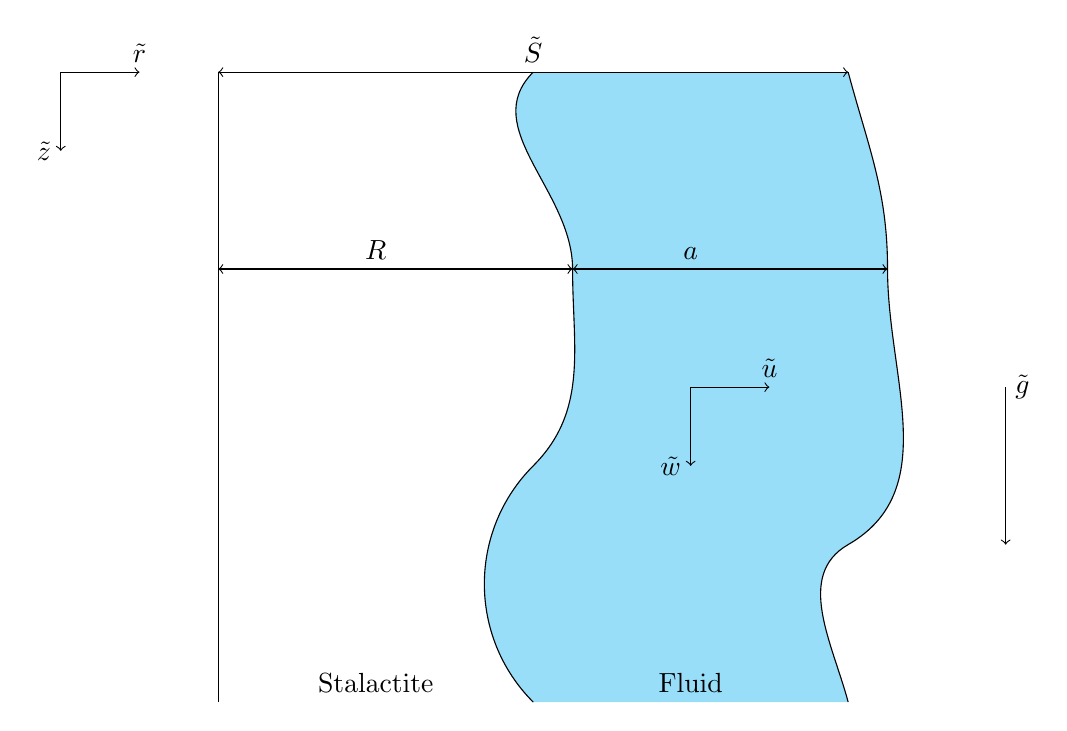
\begin{tikzpicture}
	\draw (0,0) -- (0,8);
	\fill[cyan!40!white] (4,0) to [out=135, in=-135] (4,3) to [out=45,in=-90]  (4.5,5.5) to [out=90,in=-135] (4,8) to (8,8) to [out=-75,in=90] (8.5,5.5) to [out=-90,in=30] (8,2) to [out=-150,in=105] (8,0) -- cycle;
	
	\draw (4,0) to [out=135, in=-135] (4,3) to [out=45,in=-90]  (4.5,5.5) to [out=90,in=-135] (4,8);
	\draw (8,0) to [out=105, in=-150] (8,2) to [out=30,in=-90]  (8.5,5.5) to [out=90,in=-75] (8,8);
	\draw[<->](0,5.5)--(4.5,5.5);
	\node[above] at (2,5.5) {$R$};
	\draw[<->](4.5,5.5)--(8.5,5.5);
	\node[above] at (6,5.5) {$a$};
	
	\draw[->] (6,4) --(6,3);
	\node[ left] at (6,3) {$\tilde w$};
	\draw[->] (6,4) --(7,4);
	\node[above ] at (7,4) {$\tilde u$};
	\draw[->] (10,4) --(10,2);
	\node[right] at (10,4) {$\tilde g$};
	\draw[<->] (0,8)--(8,8);
	\node[above] at (4,8) {$\tilde S$};
	\node[above] at (2,0) {Stalactite};
	\node[above] at (6,0) {Fluid};
	\draw[->] (-2,8) --(-2,7);
	\node[left] at (-2,7) {$\tilde z$};
	\draw[->] (-2,8) --(-1,8);
	\node[above] at (-1,8) {$\tilde r$};
	\end{tikzpicture}
	\caption{Geometry of the Surface of the Stalactite\label{fig:base_stalac}}
\end{figure}
For an incompressible fluid with velocity $\vec{\tilde u}=(\tilde u,0,\tilde w)$ in cylindrical coordinates $\vec{\tilde x}=(\tilde r,\tilde \theta,\tilde z)$. The continuity equation is
\begin{align}
  \pdv{\tilde u}{\tilde r}+\frac{\tilde u}{\tilde r}+\pdv{\tilde w}{\tilde z}=0 \label{continuity}
\end{align}
And the Navier Stokes Equations give
\begin{align}
  \pdv{\tilde u}{\tilde t}+\tilde u\pdv{\tilde u}{\tilde r}+\tilde w\pdv{\tilde u}{\tilde z}&=-\frac{1}{\rho}\pdv{\tilde p}{\tilde r}+\nu\left(\pdv[2]{\tilde u}{\tilde r}+\frac{1}{\tilde r}\pdv{\tilde u}{\tilde r}-\frac{1}{r^2}\tilde u+\pdv[2]{\tilde u}{\tilde z}\right)\label{navierr}\\
   \pdv{\tilde w}{\tilde t}+u\pdv{\tilde w}{\tilde r}+\tilde w\pdv{\tilde w}{\tilde z}&=-\frac{1}{\rho}\pdv{\tilde p}{\tilde z}+\nu\left(\pdv[2]{\tilde w}{\tilde r}+\frac{1}{\tilde r}\pdv{\tilde w}{\tilde r}+\pdv[2]{\tilde w}{\tilde z}\right) + g \label{navierv}
\end{align}
On the boundary between the stalactite and the fluid we have no flux and no slip i.e
\begin{align}
  \tilde u=0,\;\tilde  w=0\quad\mathrm{on}\; \tilde r=R \label{solidboundary}
\end{align}
On the surface of the fluid at $\tilde r=R+a=\tilde S(\tilde z,\tilde t)$, the kinematic boundary condition gives
\begin{align}
 \tilde   u=\pdv{\tilde S}{\tilde t}+\tilde w\pdv{\tilde S}{\tilde z} \quad\mathrm{on}\;\tilde  r=\tilde S \label{kinematic}
\end{align}
The tangential and normal stress balances on the free surface gives
\footnotesize
\begin{align}
2\pdv{\tilde S}{\tilde z}\left(\pdv{\tilde u}{\tilde r}-\pdv{\tilde w}{\tilde z}\right)+\left(1-\left(\pdv{\tilde S}{\tilde z}\right)^2\right)\left(\pdv{\tilde u}{\tilde z}+\pdv{\tilde w}{\tilde r}\right)&=0\label{tangstress}\\
  \tilde p\left(1+\left(\pdv{\tilde S}{\tilde z}\right)^2\right)-2\mu\left( \pdv{\tilde u}{\tilde r}-\pdv{\tilde S}{\tilde z}\left(\pdv{\tilde u}{\tilde z}+\pdv{\tilde w}{\tilde r}\right)+\left(\pdv{\tilde S}{\tilde z}\right)^2\pdv{\tilde w}{\tilde z}\right)&=\gamma\frac{\left(\frac{1}{\tilde S}\left(1+\left(\pdv{\tilde S}{\tilde z}\right)^2\right)-\pdv[2]{\tilde S}{\tilde z}\right)}{\left(1+\left(\pdv{\tilde S}{\tilde z}\right)^2\right)^{\frac{1}{2}}}\label{normstress}
  \end{align}
  \normalsize
  at $\tilde r= \tilde{S}$
Introduce non-dimensional variables
\small
\begin{align}
  \tilde r=Rr, \quad \tilde z=Lz, \quad\tilde  u=Uu, \quad \tilde w=Ww, \quad \tilde p=\rho Pp, \quad\tilde  t=\frac{L}{W}t,\quad \tilde S=R_0S,\quad 
\end{align}
\normalsize
Then from \eqref{continuity} we find that $U\sim \frac{WR}{L}$.
Now \eqref{continuity} becomes
\begin{align}
\pdv{ u}{ r}+\frac{ u}{ r}+\pdv{ w}{ z}=0 \label{continuityn}
\end{align}
The Non-dimensional Navier Stokes give
\begin{align}
  \pdv{ u}{ t}+ u\pdv{ u}{ r}+ w\pdv{ u}{ z}&=-\frac{P}{W^2}\frac{L^2}{{R}^2}\pdv{ p}{ r}+\frac{1}{\Re_w}\left(\frac{L^2}{{R}^2}\left(\pdv[2]{ u}{ r}+\frac{1}{ r}\pdv{ u}{ r}-\frac{1}{r^2} u\right)+\pdv[2]{ u}{ z}\right)\label{navierrn}\\
\pdv{ w}{ t}+u\pdv{ w}{ r}+ w\pdv{ w}{ z}&=-\frac{P}{W^2}\pdv{ p}{ z}+\frac{1}{\Re_w}\left(\frac{L^2}{{R}^2}\left(\pdv[2]{ w}{ r}+\frac{1}{ r}\pdv{ w}{ r}\right)+\pdv[2]{ w}{ z}\right)+ \frac{L}{W^2}g \label{naviervn}
\end{align}
where $\Re_w=\frac{WL}{\nu}$. 
\subsection{Approximations}
\subsubsection{Similar Length Scales \label{similar}}
According to Short et al \cite{short}, stalactites have regular crenulations of centimetre-scale wavelength ($L$)%\footnote{Reason why not to put $L$ large in my code}
. The radius of the stalactite ($R$) is also around 5-10 cm, so we have a similar length scale. Putting $L\sim R$ then $W\sim U$ and $\Re_w=\Re_u=\Re$ and so equations \eqref{continuityn}-\eqref{naviervn} become
\begin{align}
\pdv{ u}{ r}+\frac{ u}{ r}+\pdv{ w}{ z}&=0 \label{continuityn1}\\
\pdv{ u}{ t}+ u\pdv{ u}{ r}+ w\pdv{ u}{ z}&=-\frac{P}{U^2}\pdv{ p}{ r}+\frac{1}{\Re}\left(\pdv[2]{ u}{ r}+\frac{1}{ r}\pdv{ u}{ r}-\frac{1}{r^2} u+\pdv[2]{ u}{ z}\right)\label{navierrn1}\\
\pdv{ w}{ t}+u\pdv{ w}{ r}+ w\pdv{ w}{ z}&=-\frac{P}{U^2}\pdv{ p}{ z}+\frac{1}{\Re}\left(\pdv[2]{ w}{ r}+\frac{1}{ r}\pdv{ w}{ r}+\pdv[2]{ w}{ z}\right)+ \frac{R}{U^2}g \label{naviervn1}
\end{align}

\subsubsection{Small Reynolds Number}
According to Short et al \cite{shortshort} the Reynolds number is small enough for the Stokes approximation to be valid.
If we have a small Reynolds number the viscous terms dominate, if we balance the pressure and gravity with these so $P\sim\frac{U^2}{\Re},\; g\sim\frac{U^2}{R\Re}=\frac{U\nu}{R^2}$. So $U\sim\frac{R^2 g}{\nu}$, $P\sim gR$. So we can scale all these quantities using the known values $\rho, R, g,\nu$.
\footnotesize
\begin{align}
\tilde r=Rr, \quad \tilde z=Rz, \quad\tilde  u=\frac{R^2  g}{\nu}u, \quad \tilde w=\frac{R^2  g}{\nu}w, \quad \tilde p=\rho  g R p, \quad\tilde  t=\frac{\nu}{Rg}t,\quad \tilde S=RS
\end{align}
\normalsize
With $\Re=\frac{R^3 g}{\nu^2}$, $\Bo = \frac{\rho g L^2}{\gamma}$.  The small Reynold's number comes from the fluid flowing down the stalactite having a very small thickness. This leads to the non dimensional equations 
\begin{align}
\pdv{ u}{ r}+\frac{ u}{ r}+\pdv{ w}{ z}&=0\\\pdv[2]{ u}{ r}+\frac{1}{ r}\pdv{ u}{ r}-\frac{1}{r^2}u+\pdv[2]{ u}{ z}&=\pdv{p}{r}\\
\pdv[2]{ w}{ r}+\frac{1}{ r}\pdv{ w}{ r}+\pdv[2]{ w}{ z}&=\pdv{p}{z}-1
\end{align}

With non dimensional boundary conditions the same as \eqref{solidboundary}-\eqref{normstress} just dropping the \~{} and now without the $\mu$.
\subsubsection{Quasi-stationary Approximation}
Note that the only time dependence that we currently have is from equation \eqref{kinematic}. However since the growth of stalactites is slow \cite{short}, from here on we will set $\pdv{S}{t}=0$.
\subsection{Flow down a cylinder}
If we start by looking at a perfectly cylindrical stalactite. This means that our terms have no $z$ dependence. This will look like
\begin{figure}[H]
	\centering
	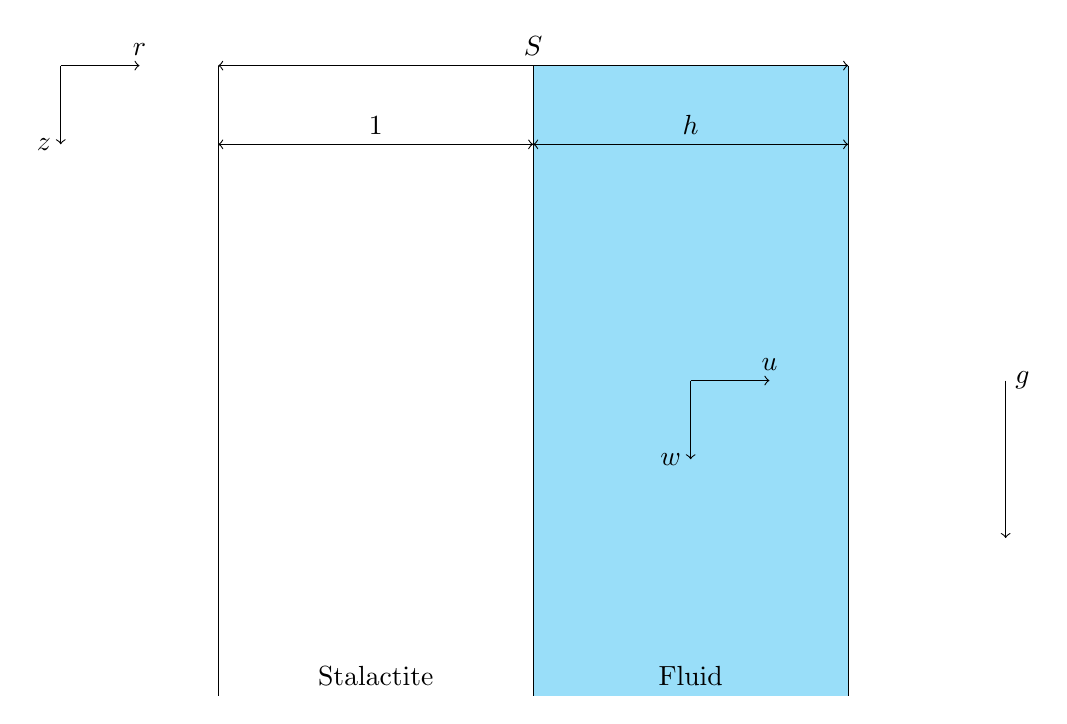
\begin{tikzpicture}
	\draw (0,0) -- (0,8);
	\fill[cyan!40!white] (4,0) rectangle (8,8);
	\draw(4,0) -- (4,8);
	\draw(8,0)--(8,8);
	\draw[<->] (0,7) --(4,7); 
	\node[above] at (2,7) {$1$};
	\draw[<->] (4,7) -- (8,7);
	\node[above] at (6,7) {$h$};
	\draw[->] (6,4) --(6,3);
\node[ left] at (6,3) {$w$};
\draw[->] (6,4) --(7,4);
\node[above ] at (7,4) {$ u$};
\draw[->] (10,4) --(10,2);
\node[right] at (10,4) {$ g$};
\draw[<->] (0,8)--(8,8);
\node[above] at (4,8) {$ S$};
\node[above] at (2,0) {Stalactite};
\node[above] at (6,0) {Fluid};
\draw[->] (-2,8) --(-2,7);
\node[left] at (-2,7) {$ z$};
\draw[->] (-2,8) --(-1,8);
\node[above] at (-1,8) {$ r$};
      \end{tikzpicture}
	\caption{Cylindrical Stalactite}
\end{figure}
The equations reduce to
\begin{align}
\pdv{r}\left(ru\right)=0\\
\pdv{p}{r}=0\\
\frac{1}{r}\pdv{r}\left(r\pdv{w}{r}\right)=-1
\end{align}
With the boundary conditions
\begin{align}
u=w=0\quad &\mathrm{on} \; r=1\\
\begin{drcases}
u&=0\\
\pdv{w}{r}&=0\\
p-2\pdv{u}{r}&=\frac{\gamma}{S}
\end{drcases}
\quad& \mathrm{on} \; r=S=1+\frac{a}{R}=1+h
\end{align}
Integrating the equations and making them satisfy the boundary conditions gives us
\begin{align}
u&=0\label{baseu}\\
w&=\frac{1}{4}\left(1-r^2+2S^2\log r\right)\label{basew}\\
p&=\frac{\gamma}{ S}\label{basep}
\end{align}
\subsection{Perturbing the Surface\label{perturb}}
Now we know the flow for a cylindrical stalactite, however stalactites have crenulations on them. In this section we will be analysing what effect small changes in the shape of the radius has on the flow of the fluid. If we introduce these crenulations as a small change in the radius $\delta \tilde r$ from the base cylindrical case then this should affect the flow as follows 
\begin{align}
u&=U(r)+\delta \tilde u(r,z)\label{eq:perturbtop}\\
w&=W(r)+\delta\tilde w(r,z)\\
p&=P(r)+\delta\tilde p(r,z)\\
\end{align}
With the fluid now in the region
\begin{align}
1+\delta\tilde r(z)\leq r\leq S+\delta \tilde s(z) \label{eq:perturbbottom}
\end{align}
The stalactite starts to look more like what would be expected.
\begin{figure}[H]
	\centering
	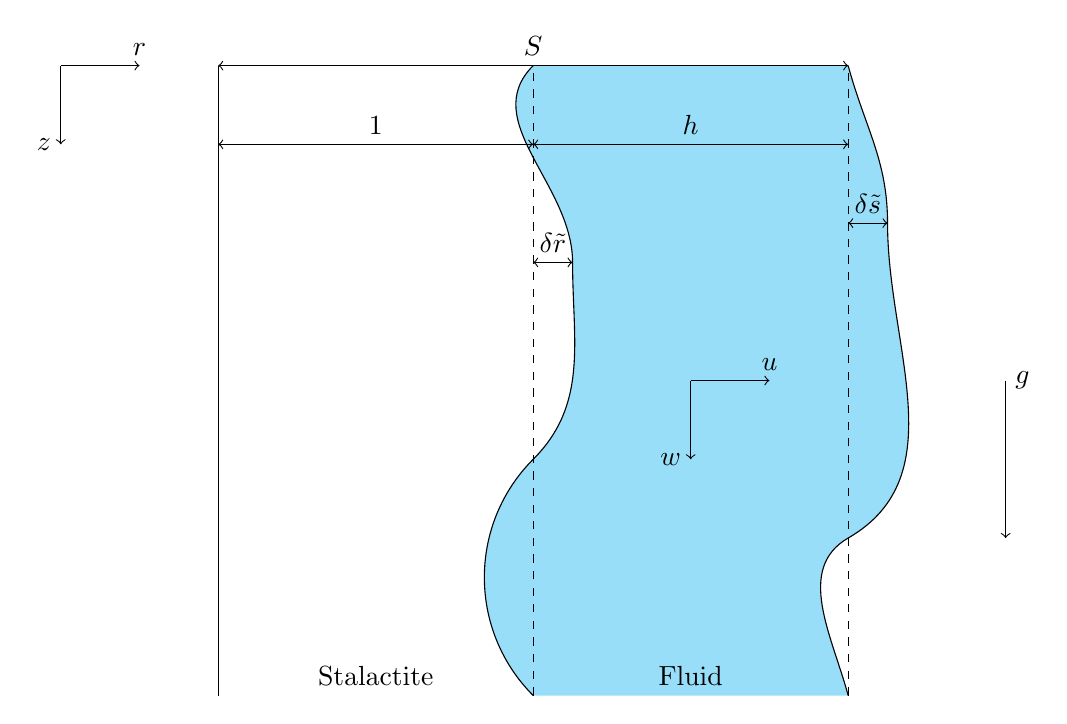
\begin{tikzpicture}
	\draw (0,0) -- (0,8);
	\fill[cyan!40!white] (4,0) to [out=135, in=-135] (4,3) to [out=45,in=-90]  (4.5,5.5) to [out=90,in=-135] (4,8) to (8,8) to [out=-75,in=90] (8.5,6) to [out=-90,in=30] (8,2) to [out=-150,in=105] (8,0) -- cycle;
	\draw[dashed](4,0) -- (4,8);
	\draw[dashed](8,0)--(8,8);
	\draw (4,0) to [out=135, in=-135] (4,3) to [out=45,in=-90]  (4.5,5.5) to [out=90,in=-135] (4,8);
	\draw (8,0) to [out=105, in=-150] (8,2) to [out=30,in=-90]  (8.5,6) to [out=90,in=-75] (8,8);
	\draw[<->](4,5.5)--(4.5,5.5);
	\node[above] at (4.25,5.5) {$\delta\tilde r$};
	\draw[<->](8,6)--(8.5,6);
	\node[above] at (8.25,6) {$\delta \tilde s$};
	\draw[<->] (0,7) --(4,7); 
	\node[above] at (2,7) {$1$};
	\draw[<->] (4,7) -- (8,7);
	\node[above] at (6,7) {$h$};
	\draw[->] (6,4) --(6,3);
\node[ left] at (6,3) {$w$};
\draw[->] (6,4) --(7,4);
\node[above ] at (7,4) {$ u$};
\draw[->] (10,4) --(10,2);
\node[right] at (10,4) {$ g$};
\draw[<->] (0,8)--(8,8);
\node[above] at (4,8) {$ S$};
\node[above] at (2,0) {Stalactite};
\node[above] at (6,0) {Fluid};
\draw[->] (-2,8) --(-2,7);
\node[left] at (-2,7) {$ z$};
\draw[->] (-2,8) --(-1,8);
\node[above] at (-1,8) {$ r$};
	\end{tikzpicture}
	\caption{Stalactite with Crenulations\label{sta_cren}}
\end{figure}

Looking at the $O(1)$ terms, we find that we get the same dynamics as \eqref{baseu}-\eqref{basep}.
\begin{align}
U&=0\label{baseu1}\\
W&=\frac{1}{4}\left(1-r^2+2S^2\log r\right)\label{basew1}\\
P&=\frac{\gamma}{ S}\label{basep1}
\end{align}
Looking at the $O(\delta)$ terms we get 
\begin{align}
\frac{1}{r}\pdv{r}\left(r\tilde u\right)+\pdv{\tilde w}{z}&=0\label{smallconttop}\\
\frac{1}{r}\pdv{r}\left(r\pdv{\tilde u}{r}\right)-\frac{1}{r^2}\tilde u+\pdv[2]{\tilde u}{z}&=\pdv{\tilde p}{r}\\
\frac{1}{r}\pdv{r}\left(r\pdv{\tilde w}{r}\right)+\pdv[2]{\tilde w}{z}&=\pdv{\tilde p}{z}\label{smallcontbottom}
\end{align}
with boundary conditions
\begin{align}
\tilde r \eval{\dv{U}{r}}_1+\eval{\tilde u}_1&=0\\
\tilde r \eval{\dv{W}{r}}_1+\eval{\tilde w}_1&=0\\
\eval{\tilde u}_{S}-\eval{W}_{S}\dv{\tilde s}{z}&=0\\
\tilde s\eval{\dv[2]{W}{r}}_{S} +\eval{\pdv{\tilde u}{z}}_{S}+\eval{\pdv{\tilde w}{r}}_{S}&=0\\
\eval{\dv{P}{r}}_{S}+\eval{\tilde p}_{S}-2\eval{\pdv{\tilde u}{r}}_{S}+\dv{\tilde s}{z}\eval{\dv{W}{r}}_{S}+\frac{\gamma\tilde s}{ S^2}+\gamma\dv[2]{\tilde s}{z}&=0
\end{align}
If we substitute the know values for $P,U,W$ into these equations we get 
\begin{align}
\eval{\tilde u}_1&=0\label{boundarytop}\\
\eval{\tilde w}_1&= \frac{1}{2}\left(1-S^2\right)\tilde r\\
\eval{\tilde u}_{S}&=\frac{1}{4}\left(1-S^2+2S^2\log S\right)\dv{\tilde s}{z}\\
\eval{\pdv{\tilde u}{z}}_{S}+\eval{\pdv{\tilde w}{r}}_{S}&=\tilde s\\
\eval{\tilde p}_{S}-2\eval{\pdv{\tilde u}{r}}_{S}&=-\gamma\left(\frac{\tilde s}{S^2}+\dv[2]{\tilde s}{z}\right)\label{boundarybottom}
\end{align}
To solve this problem, we will follow similar steps to works by Papageorgiou \cite{doi:10.1063/1.857784} and Pekeris \cite{pekeris48}. If we introduce a stream-function $\phi$, defined by
\begin{align}
\tilde u=\frac{1}{r}\pdv{\psi}{z},\quad \tilde w=-\frac{1}{r}\pdv{\psi}{r}
\end{align}
Now \eqrefs{smallcont} become
\begin{align}
\frac{1}{r}\pdv[2]{\psi}{r}{z}-\frac{1}{r}\pdv[2]{\psi}{z}{r}&=0\\
\frac{1}{r^3}\psi_{z}-\frac{1}{r^2}\psi_{zr}+\frac{1}{r}\psi_{zrr}-\frac{1}{r^3}\psi_z +\frac{1}{r}\psi_{zzz}&=p_r\label{psi1}\\
-\frac{1}{r^3}\psi_{r}+\frac{1}{r^2}\psi_{rr}-\frac{1}{r}\psi_{rrr}-\frac{1}{r}\psi_{rzz}&=p_z\label{psi2}
\end{align}
%potentially corrected to here
Where $\psi_r=\pdv{\psi}{r}$. We have reduced the number of equations to solve from 3 to 2, and by cross differentiating \eqref{psi1} and \eqref{psi2} and equating $p_{rz}$ gives us the single equation.
\small
\begin{align}
-{\frac{1}{r^2}\psi_{zzr}}+{\frac{1}{r}\psi_{zzrr}}+\frac{1}{r}\psi_{zzzz}-\frac{3}{r^4}\psi_r+\frac{3}{r^3}\psi_{rr}-\frac{2}{r^2}\psi_{rrr}+\frac{1}{r}\psi_{rrrr}-\frac{1}{r^2}\psi_{rzz}+\frac{1}{r}\psi_{rrzz}=0 \label{streamnav}
\end{align}
\normalsize
Taking the Fourier transform of the $z$ component.
\begin{align}
\phi(r,k)&=\int_{-\infty}^{\infty}\psi(r,z)e^{-ikz}\dd{z}\\
\hat r(k)&=\int_{-\infty}^{\infty}\tilde r(z)e^{-ikz}\dd{z}\\
\hat s(k)&=\int_{-\infty}^{\infty}\tilde s(z)e^{-ikz}\dd{z}\\
\hat p(r,k)&=\int_{-\infty}^{\infty}\tilde p(r,z)e^{-ikz}\dd{z}
\end{align}
where all perturbations disappear in the far field, so 
\begin{align}
\F\left[\dv{f}{z}\right]&=\int_{-\infty}^{\infty}\dv{f}{z}e^{-ikz}\dd{z}\\
&=\left[f(z)e^{-ikz}\right]^\infty_{-\infty} +ik\int_{-\infty}^{\infty}fe^{-ikz}\dd{z}\\
&=ik\F[f(z)]
\end{align}
Equation \eqref{streamnav} becomes
\begin{align}
\phi_{rrrr}-\frac{2}{r}\phi_{rrr}+\frac{3}{r^2}\phi_{rr}-\frac{3}{r^3}\phi_r-k^2\left(2\phi_{rr}-\frac{2}{r}\phi_{r}\right)+k^4\phi=0\label{phiclose}
\end{align}
This can be rewritten as 
\begin{align}
r\pdv{r}\left(\frac{1}{r}\pdv{r}\left[r\pdv{r}\left(\frac{1}{r}\pdv{r}\phi\right)\right]\right)-2k^2r\pdv{r}\left(\frac{1}{r}\pdv{r}\phi\right)+k^4\phi&=0\\
\mathcal{D}^4\phi&=0
\end{align}
where \begin{align}\D^2&=r\pdv{r}\left(\frac{1}{r}\pdv{r}\right)-k^2\\&=\pdv[2]{r}-\frac{1}{r}\pdv{r}-k^2\end{align}
If we let $\D^2\phi=\chi$ then $\D^2\chi=0$. Now letting $\chi=r\tilde\chi$
\begin{align}
\pdv{\chi}{r}&=r\pdv{\tilde\chi}{r}+\tilde\chi\\
\pdv[2]{\chi}{r}&=r\pdv[2]{\tilde\chi}{r}+2\pdv{\tilde\chi}{r}
\end{align}
Then
\begin{align}
\D^2\chi&=r\pdv[2]{\tilde\chi}{r}+2\pdv{\tilde\chi}{r}-\pdv{\tilde\chi}{r}-\frac{1}{r}\tilde\chi-k^2r\tilde\chi\\
&=r\pdv[2]{\tilde\chi}{r}+\pdv{\tilde\chi}{r}-\left(\frac{1}{r}+k^2r\right)\tilde\chi\
\end{align}
If we now let $kr=x$, we get
\begin{align}
\frac{x}{k}\D^2\chi=x^2\pdv[2]{\tilde\chi}{x}+x\pdv{\tilde\chi}{x}-\left(1+x^2\right)\tilde\chi
\end{align}
which is the modified Bessel Equation.
\begin{align}
x^2\pdv[2]{\tilde\chi}{x}+x\pdv{\tilde\chi}{x}-\left(1+x^2\right)\tilde\chi=0
\end{align}
This has solutions 
\begin{align}
\tilde\chi=AI_1(x)+BK_1(x)
\end{align}
So now
\begin{align}
\D^2\phi=\frac{x}{k}(AI_1(x)+BK_1(x))
\end{align} If we let $\phi=r\tilde\phi$, doing similar things we find
\begin{align}
x^2\pdv[2]{\tilde\phi}{x}+x\pdv{\tilde\phi}{x}-\left(1+x^2\right)\tilde\phi=\frac{x^2}{k^2}\left(AI_1(x)+BK_1(x)\right)\label{phibessel}
\end{align}
We can solve this by finding a homogeneous solution and the particular one. The homogeneous equation is again the modified Bessel equation, meaning the homogenous solution is
\begin{align}
\tilde\phi_{H}=CI_1(x)+DK_1(x)
\end{align}
in order to find the particular solution we can use variation of parameters. This is done by saying that the particular solution will be of the form.
\begin{align}
\tilde\phi_p=f(x)I_1(x)+g(x)K_1(x)
\end{align}
Where we set 
\begin{align}
\pdv{f}{x}I_1+\pdv{g}{x}K_1=0\label{vpc1}
\end{align}
Now
\begin{align}
\pdv{\tilde\phi}{x}&=f\dv{I_1}{x}+g\dv{K_1}{x}\\\pdv[2]{\tilde\phi}{x}&=\pdv{f}{x}\dv{I_1}{x}+f\dv[2]{I_1}{x}+\pdv{g}{x}\dv{K_1}{x}+g\dv[2]{K_1}{x}
\end{align}
Substituting these into \eqref{phibessel} and noting that, by definition, $I_1,\;K_1$ satisfy this modified Bessel equation, we find
\begin{align}
\pdv{f}{x}\dv{I_1}{x}+\pdv{g}{x}\dv{K_1}{x}=\frac{A}{k^2}I_1+\frac{B}{k^2}K_1=\frac{\tilde\chi}{k^2}\label{vpc2}
\end{align}
We can solve the simultaneous equations \eqref{vpc1} and \eqref{vpc2} and integrate to get
\begin{align}
f(x,k)&=\int_k^x{\frac{\tilde\chi(y)K_1(y)}{k^2W(y)}\dd{y}}\\
 g(x,k)&=-\int_k^x{\frac{\tilde\chi(y)I_1(y)}{k^2W(y)}\dd{y}}
\end{align}
where $W$ is the Wronskian
\begin{align}
W=\dv{I_1}{x}K_1-I_1\dv{K_1}{x}
\end{align}
Using properties of modified Bessel functions we find
\begin{align}
W(y)&=I_1'(y)K_1(y)-I_1(y)K_1'(y)\\
&=\left(I_0(y)-\frac{1}{y}I_1(y)\right)K_1(y)+I_1(y)\left(K_0(y)+\frac{1}{y}K_1(y)\right)\\
&=I_0(y)K_1(y)+I_1(y)K_0(y)\\&=\frac{1}{y}
\end{align}
The overall solution is the sum of the homogenous and particular solutions.
\begin{align}
\tilde\phi(x)&=(C+f(x))I_1(x)+(D+g(x))K_1(x)
\end{align}
To work out the constants we need to substitute in the boundary conditions. To do this it is helpful to know what the boundary conditions are in terms of $\tilde\phi$. For this we will need to find $\hat u,\;  \hat w$, the Fourier transform of $\tilde u,\;  \tilde w$, in terms of $\tilde\phi$.
\begin{align}
\hat u%&=\frac{1}{r}\pdv{\psi}{z}\\
%&=ik\frac{1}{r}\phi\\
&=ik\tilde\phi(x)\\
\hat w%&=-\frac{1}{r}\pdv{\psi}{r}\\
%&=-\frac{1}{r}\pdv{r}(r\tilde \phi)\\
&=-\frac{k}{x}\tilde\phi(x)-k\tilde\phi'(x)
\\\pdv{\hat u}{z}&=-k^2\tilde\phi(x)\\
\pdv{\hat u}{r}&=ik^2\tilde\phi'(x)\\
\pdv{\hat w}{r}&=k^2\left(\frac{\tilde\phi(x)}{x^2}-\frac{\tilde\phi'(x)}{x}-\tilde\phi''(x)\right)
\end{align}
We can get $\hat p$ in terms of $\tilde\phi$ by taking the Fourier transform of \eqref{psi2}.
\begin{align}
\hat p\left(\frac{x}{k}\right)=ik^2\left(\left(\frac{1}{x^3}-\frac{1}{x}\right)\tilde\phi-\left(1+\frac{1}{x^2}\right)\tilde \phi'+\frac{2}{x}\tilde\phi''+\tilde\phi'''\right)
\end{align}
Therefore the boundary conditions, equations \eqrefs{boundary} can be written as
\begin{align}
\tilde\phi(k)&=0\label{phi1}\\
\tilde\phi'(k)&=\frac{1}{2k}\left(S^2-1\right)\hat r\label{phi2}\\
\tilde\phi(\sigma)&=\frac{1}{4}\left(1-S^2+2S^2\log S\right)\hat{s}\label{phi3}
\end{align}
\begin{align}
(\sigma^2-1)\tilde\phi(\sigma)+\sigma\tilde\phi'(\sigma)+\sigma^2\tilde\phi''(\sigma)&=-S^2\hat s\label{phi4}\\
\left(1- \sigma^2\right)\tilde\phi(\sigma)-(3\sigma^3+\sigma)\tilde\phi'(\sigma)+2\sigma^2\tilde\phi''(\sigma)+\sigma^3\tilde\phi'''(\sigma)&=i\gamma(\sigma-\sigma^3)\hat s \label{phi5}
\end{align}
where $\sigma=kS$. The boundary conditions contain the first three derivates of $\tilde\phi$, which are
\begin{align}
\tilde\phi'%&=(C+f)I_1'+(D+g)K_1'+f'I_1+g'K_1\\
%&=(C+f)I_1'+(D+g)K_1'+x\tilde\chi K_1I_1-x\tilde\chi I_1K_1\\
&=(C+f)I_1'+(D+g)K_1'\\
\tilde\phi''%&=(C+f)I_1''+(D+g)K_1''+f'I_1'+g'K_1'\\
%&=(C+f)I_1''+(D+g)K_1''+\frac{\tilde\chi}{k^2}\\
&=(C+f)\left(\left(1+\frac{1}{x^2}\right)I_1-\frac{1}{x}I_1'\right)+(D+g)\left(\left(1+\frac{1}{x^2}\right)K_1-\frac{1}{x}K_1'\right)+\frac{\tilde\chi}{k^2}\\
\tilde\phi'''& =\left(1+\frac{3}{x^2}\right)\left[(C+f)\left(I_1'-\frac{I_1}{x}\right)+(D+g)\left(K_1'-\frac{K_1}{x}\right)\right] +\frac{1}{k^2}\left(\tilde\chi'-\frac{\tilde\chi}{x}\right)
\end{align}
Note as we have written these in terms of the modified Bessel functions and the first derivatives, we find
\begin{align}
\tilde\phi'' & = \left(1+\frac{1}{x^2}\right)\tilde\phi-\frac{1}{x}\tilde\phi' + \frac{\tilde\chi}{k^2}\\
\tilde\phi'''& =  \left(1+\frac{3}{x^2}\right)\left(\tilde\phi'-\frac{\tilde\phi}{x}\right)+ \frac{1}{k^2}\left(\tilde\chi'-\frac{\tilde\chi}{x} \right)
\end{align}
So the stress balance equations \eqref{phi4}-\eqref{phi5} can be rewritten as
\begin{align}
2\sigma^2\tilde\phi(\sigma) + S^2\tilde\chi(\sigma)&= -S^2\hat s\label{phi4_good}\\
2\sigma^2\tilde\phi'(\sigma)-\frac{1}{k^2}\left(\sigma\tilde\chi(\sigma)+\sigma^2\tilde\chi'(\sigma) \right)\label{phi5_good} & = i\gamma(\sigma^2-1)\hat s
\end{align}

From the no flux condition, equation \eqref{phi1} we find 
\begin{align}
D=-\frac{CI_1(k)}{K_1(k)}
\end{align}

Looking at the no slip condition, equation \eqref{phi2} we get
\begin{align}
C\left(I_1'(k)-\frac{I_1(k)}{K_1(k)}K_1'(k)\right)=\frac{1}{2k}(S^2-1)\hat r\\
C=\frac{K_1(k)}{2}(S^2-1)\hat r
\end{align}
So far we have
\footnotesize
\begin{align}
\sq{\tilde\phi=\left(\frac{K_1(k)(S^2-1)}{2}\hat r+\int_k^x{\frac{y\tilde\chi(y)K_1(y)}{k^2}\dd{y}}\right)I_1(x)-\left(\frac{I_1(k)(S^2-1)}{2}\hat r+\int_k^x{\frac{y\tilde\chi(y)I_1(y)}{k^2}\dd{y}}\right)K_1(x)}
\end{align}
\normalsize
Now we will evaluate these integrals using some of the properties of Bessel functions\cite[Sections 10.28-29]{NIST:DLMF}.

Let $\tilde{\mb_n}, \hat{\mb_n}$ be $I_n$ or $e^{in\pi}K_n$
\begin{align}
\int{x\tilde{\mb_1}(x) \hat{\mb_1}(x)\dd{x}}=\frac{x^2}{2}\tilde{\mb_1}(x) \hat{\mb_1}(x)-\int{\frac{x^2}{2}(\tilde{\mb_1}'(x) \hat{\mb_1}(x)+\tilde{\mb_1}(x) \hat{\mb_1}'(x))\dd{x}}
\end{align}
We can write $\mb_1(x)=\mb_0'(x)$
\begin{align}
\int{x^2\tilde{\mb_1}'(x) \hat{\mb_1}(x)\dd{x}}&=\int{x^2\tilde{\mb_0}''(x) \hat{\mb_1}(x)\dd{x}}\\
&=\int{x^2\tilde{\mb_0}(x) \hat{\mb_1}(x)\dd{x}}-\int{x\tilde{\mb_0}'(x) \hat{\mb_1}(x)\dd{x}}
\end{align}
\begin{align}
\int{x^2(\tilde{\mb_0}(x) \hat{\mb_1}(x)+\tilde{\mb_1}(x) \hat{\mb_0}(x))\dd{x}}&=\int{x^2(\tilde{\mb_0}(x) \hat{\mb_0}'(x)+\tilde{\mb_0}'(x) \hat{\mb_0}(x))\dd{x}}\\
&=x^2\tilde{\mb_0}(x) \hat{\mb_0}(x)-2\int{x\tilde{\mb_0}(x) \hat{\mb_0}(x)\dd{x}}
\end{align}

\begin{align}
\int{x\tilde{\mb_0}(x) \hat{\mb_0}(x)\dd{x}}=x\tilde{\mb_1}(x) \hat{\mb_0}(x)-\int{x\tilde{\mb_1}(x) \hat{\mb_0}'(x)\dd{x}}
\end{align}
Putting this all together we get
\footnotesize
\begin{align}
\sq{\int{x\tilde{\mb_1}(x) \hat{\mb_1}(x)\dd{x}}=\frac{1}{2}\left(x^2\left(\tilde{\mb_1}(x) \hat{\mb_1}(x)-\tilde{\mb_0}(x) \hat{\mb_0}(x)\right)+x\left(\tilde{\mb_1}(x) \hat{\mb_0}(x)+\tilde{\mb_0}(x) \hat{\mb_1}(x)\right)\right)}
\end{align}
\normalsize
The three integrals that we require are
\footnotesize
\begin{align}
\int{xI_1^2(x)\dd{x}}&=\frac{x^2}{2}\left(I_1^2(x)-I_0^2(x)\right)+ xI_1(x)I_0(x)& \equiv C_1(x)\\
\int{xK_1^2(x)\dd{x}}&=\frac{x^2}{2}\left(K_1^2(x)-K_0^2(x)\right) - xK_1(x)K_0(x)& \equiv C_2(x)\\
\int{xI_1(x)K_1(x)\dd{x}}&=\frac{1}{2}\left(x^2(I_1(x)K_1(x)+I_0(x)K_0(x))+x(I_0(x)K_1(x)-I_1(x)K_0(x))\right)&\equiv C_3(x)
\end{align}
\normalsize
This gives
\footnotesize
\begin{align}
\tilde\phi&=\begin{pmatrix}\frac{A}{k^2}& \frac{B}{k^2} & \hat r\end{pmatrix}\begin{pmatrix}\frac{x}{2}I_0(x)-\left(\frac{1}{2}+C_3(k)\right)I_1(x)+C_1(k)K_1(x)\\\left(C_3(k)-\frac{1}{2}\right)K_1(x)-\frac{x}{2}K_0(x)-C_2(k)I_1(x)\\\frac{1}{2}(I_1(x)K_1(k)-I_1(k)K_1(x))(S^2-1)\end{pmatrix}\\
\tilde\phi'&=\begin{pmatrix}\frac{A}{k^2}& \frac{B}{k^2} & \hat r\end{pmatrix}\begin{pmatrix}\frac{1}{2}\left(x+2C_3(k)+\frac{1}{x}\right)I_1(x)-C_3(k)I_0(x)-C_1(k)K_0(x)-\frac{C_1(k)}{x}K_1(x)\\\frac{1}{2}\left(x-2C_3(k)+\frac{1}{x}\right)K_1-C_3(k)K_0-C_2(k)I_0(x)+\frac{C_2(k)}{x}I_1(x)\\\left(K_1(k)I_0(x)-\frac{1}{x}I_1(x)K_1(k)+I_1(k)K_0(x)+ \frac{1}{x}I_1(k)K_1(x)\right)\frac{(S^2-1)}{2}\end{pmatrix}
\end{align}
\normalsize
Therefore we can express the boundary conditions of the fluid-air interface, equations \eqref{phi3}, \eqref{phi4_good} and \eqref{phi5_good} as a linear system of equations, which can be written in the form
\begin{align}
M\begin{pmatrix}
A \\ B \\ \hat{s}
\end{pmatrix}= \vec{v}\hat{r}
\end{align}
where $M$ and $\vec{v}$ are found by rearranging equations \eqref{phi3}, \eqref{phi4_good} and \eqref{phi5_good} into that form. This matrix can be inverted and so we can find that Fourier transform of the surface perturbation.
\begin{align}
\hat{s} = \alpha(k;S,\gamma)\hat{r}
\end{align}
 where $\alpha = (M^{-1}\vec{v})_3$. I have used the syms package in MATLAB to invert the matrix and find $\alpha$.
%From \eqref{phi3} we get
%\begin{align}
%\frac{1}{4}\left(S^2-1-2S^2\log S\right)\hat{s}=&\frac{J(\sigma,k)(1-S^2)}{2}\hat r+\int_k^{\sigma}{\frac{y\left(AI_1(y)+BK_1(y)\right)J(\sigma,y)}{k^2}\dd{y}}
%\end{align}
%where 
%\begin{align}
%J(a,b)=I_1(a)K_1(b)-I_1(b)K_1(a)
%\end{align}
%Then
%\begin{align}
%B=\frac{1}{b_0}(b_1\hat r + b_2 \hat s + b_3A)
%\end{align}
%where
%\begin{align}
%b_0 &= \int_k^{\sigma}{\frac{yK_1(y)J(\sigma,y)}{k^2}\dd{y}}\\
%b_1 & = \frac{(S^2-1)J(\sigma,k)}{2}\\
%b_2& = \frac{1}{4}(S^2- 1- 2S^2\log S)\\
%b_3 &  = -\int_k^{\sigma}{\frac{yI_1(y)J(\sigma,y)}{k^2}\dd{y}}
%\end{align}
%
%Define
%\begin{align}
%W(a,b)=I_1'(a)K_1(b)-I_1(a)K_1'(b)
%\end{align}
%From \eqref{phi4} we get
%\begin{align}
%\frac{\left(AI_1(y)+BK_1(y)\right)}{k^2}+ \frac{(1-S^2)J(\sigma,k)}{2}+\int_k^{\sigma}{\frac{y\left(AI_1(y)+BK_1(y)\right)J(\sigma,y)}{k^2}\dd{y}} = S^2\hat s
%\end{align}
%
%\begin{align}
%a_1=&\int_k^{kS}{\frac{I_1(y)-\gamma K_1(y)}{W(y)}\left(\left(\frac{1}{S^2}-1\right)J^1(kS,y)-k^2J^2(kS,y)\right)\dd{y}}-k^2(I_1(kS)-\gamma K_1(kS)\\
%a_2=&\frac{1}{4}(1-S^2+2S^2\log S)\hat s+k^2\beta K_1(kS)-\frac{(S^2-1)\hat r}{2kW(k)}\left(\left(\frac{1}{S^2}-1\right)J^1(kS,k)-k^2J^2(kS,k)\right)\nonumber\\
%&-\int_k^{kS}{\frac{\beta K_1(y)}{W(y)}\left(\left(\frac{1}{S^2}-1\right)J^1(kS,y)-k^2J^2(kS,y)\right)\dd{y}}
%\end{align}
%Note so far we have
%\begin{align}
%A&=a_1\bar s+a_2\bar r +a_3\\
%B&=b_1\bar s +b_2\bar r +b_3\\
%C&=c_1 \bar r\\
%D&=d_1 \bar r
%\end{align}
%So from the pressure equation we'll get
%\begin{align}
%\alpha_1 \bar s=\alpha_2 A +\alpha_3 B+\alpha_4 C + \alpha_5 D
%\end{align}
%which means we can write 
%\begin{align}
%\bar s =\beta_1\bar r +\beta_2 
%\end{align}
%If we introduce the vectors
%\begin{align}
%\vb{A}&=\begin{pmatrix}
%A\\ B
%\end{pmatrix}\\
%\vb{C}&=\begin{pmatrix}
%C\\D
%\end{pmatrix}\\
%\vb{v}(x)&=\begin{pmatrix}
%I_1(x)\\K_1(x)
%\end{pmatrix}\\
%M(x)&=\begin{pmatrix}
%\int_k^{x}{\frac{I_1(y)K_1(y)}{W(y)}\dd{y}}&-\int_k^{x}{\frac{I_1(y)I_1(y)}{W(y)}\dd{y}}\\
%\int_k^{x}{\frac{K_1(y)K_1(y)}{W(y)}\dd{y}}&-\int_k^{x}{\frac{I_1(y)K_1(y)}{W(y)}\dd{y}}
%\end{pmatrix}
%\end{align}
%So now 
%\begin{align}
%\tilde\phi(x)&=\vb{C}^{T}\vb{v}(x)+\vb{A}^TM(x)\vb{v}(x)\\
%\tilde\phi'(x)&=\vb{C}^{T}\vb{v}'(x)+\vb{A}^TM(x)\vb{v}'(x)\\
%\tilde\phi''(x)&=\vb{C}^{T}\vb{v}''(x)+\vb{A}^TM(x)\vb{v}''(x)+\vb{A}^T\vb{v}(x)\\
%\tilde\phi'''(x)&=\vb{C}^{T}\vb{v}'''(x)+\vb{A}^TM(x)\vb{v}'''(x)+\vb{A}^TM'(x)\vb{v}''(x)+\vb{A}^T\vb{v}'(x)
%\end{align}
%
%\begin{align}
%\vb{A}^TM(x)\vb{v}(x)&=A\left(M_{11}(x)I_1(x)+M_{12}(x)K_1(x)\right)+B\left(M_{21}(x)I_1(x)+M_{22}K_1(x)\right)
%\end{align}
%Doing this we find that 
%\begin{align}
%\phi=&\frac{1}{2}AxI_0(x)-\frac{1}{2}BxK_0(x)\\&+\left[C-\left[\frac{k^2}{2}\left(I_1(k)K_1(k)+I_0(k)K_0(k)\right)+kI_0(k)K_1(k)\right]A-\left[\frac{k^2}{2}\left(K_1^2(k)-K_0^2(k)\right)-kK_1(k)K_0(k)\right]B\right]I_1(x)\\
%&+\left[D+\left[\frac{k^2}{2}\left(I_1^2(k)-I_0^2(k)\right)+kI_1(k)I_0(k)\right]A+\left[\frac{k^2}{2}\left(I_1(k)K_1(k)+I_0(k)K_0(k)\right)+kI_0(k)K_1(k)\right]B\right]K_1(x)
%\end{align}
\subsubsection{An alternative approach}
Here we are going to use the properties of Bessel functions, which can be found in appendix \ref{Bessel}, in order to solve the equation. This was inspired by the method used by Mestel \cite{mestel_1996}.
Writing \eqrefs{smallcont} as
\begin{align}
\grad \cdot\vb{u}&=0\\
\grad^2\vb{u}&=\grad p \label{stokes}
\end{align}
Taking the divergence of \eqref{stokes} we get
\begin{align}
\grad^2p=0 \label{lapacep}
\end{align}
Taking the Fourier transform of equation \ref{lapacep} gives
\begin{align}
\D^2_0 \hat{p}=0
\end{align}
where $\Db$ is defined in \eqref{besselo}. This modified Bessel equation has the solution.
\begin{align}
\hat{p}=AI_0(x)+BK_0(x)
\end{align}
Taking the Fourier transform of equation \eqref{stokes} and substituting in this expression for $\hat p$ gives us the equations.
\begin{align}
D^2_1\hat{u}&=\frac{Ax^2}{k}I_1(x)-\frac{Bx^2}{k}K_1(x)\\
D^2_0\hat{w}&=\frac{iAx^2}{k}I_0(x)+\frac{iBx^2}{k}K_0(x)
\end{align}
The solution to these equations are
\begin{align}
u(x)&=\left(F-\frac{A}{2k}\right)I_1(x)+\left(G+\frac{B}{2k}\right)K_1(x)+\frac{Ax}{2k}I_0(x)+\frac{Bx}{2k}K_0(x)\\
w(x)&=CI_0(x)+DK_0(x)+\frac{iAx}{2k}I_1(x)-\frac{iBx}{2k}K_1(x)
\end{align}
The method for finding these solutions can be found in appendix \ref{Bessel}. To find the values of the constants we make use of the boundary conditions and the incompressibility condition. From the incompressibility condition $\grad\cdot\vb{u}=0$
\begin{align}
u(x)&=-\left(iC+\frac{A}{k}\right)I_1(x)+\left(iD+\frac{B}{k}\right)K_1(x)+\frac{Ax}{2k}I_0(x)+\frac{Bx}{2k}K_0(x)\\
w(x)&=CI_0(x)+DK_0(x)+\frac{iAx}{2k}I_1(x)-\frac{iBx}{2k}K_1(x)
\end{align}
From the boundary conditions, equations \eqrefs{boundary} we find.
\footnotesize
\begin{align}
-\left(iC+\frac{A}{k}\right)I_1(k)+\left(iD+\frac{B}{k}\right)K_1(k)+\frac{A}{2}I_0(k)+\frac{B}{2}K_0(k)&=0\\
CI_0(k)+DK_0(k)+\frac{iA}{2}I_1(k)+\frac{iB}{2}K_1(k)&=\frac{1}{2}(1-S^2)\hat r\\
\left(iD+\frac{B}{k}\right)K_1(kS)-\left(iC+\frac{A}{k}\right)I_1(kS)+\frac{AS}{2}I_0(kS)+\frac{BS}{2}K_0(kS)&=\frac{ik}{4}(1-S^2+2S^2\log S)\hat{s}\\
(2kC-iA)I_1(kS)+(iB-2kD)K_1(kS)+ik[SAI_0(kS)+SBK_0(kS)]&=-\hat s\\
(A+2ikC)I_0(kS)-\frac{1}{kS}((2+(kS)^2)A+2ikC)I_1(kS)&\nonumber\\+(B+2ikD)K_0(kS)+\frac{1}{kS}((2-(kS)^2)B+2ikD)K_1(kS)&=\frac{\gamma}{S^2}(k^2S^2-1)\hat s
\end{align}
\normalsize
We can solve this linear system of equation to find again that $\hat s =\alpha(k) \hat{r}$, where $\alpha(-k)=\alpha^*(k)$ for $s$ to be real. 


\end{document}
